%%%%%%%%%%%%%%%%%%%%%%%%%%%%%%%%%%%%%%%%%%%%%%%%%%%%%%%%%%%%%%%%%%%%%%%%%%%%%%%%
%2345678901234567890123456789012345678901234567890123456789012345678901234567890
%        1         2         3         4         5         6         7         8

%\documentclass[letterpaper, 10 pt, conference]{ieeeconf}  % Comment this line out if you need a4paper
\documentclass[conference]{IEEEtran}
%\documentclass[a4paper, 10pt, conference]{ieeeconf}      % Use this line for a4 paper

\IEEEoverridecommandlockouts                              % This command is only needed if
                                                          % you want to use the \thanks command

%\overrideIEEEmargins                                      % Needed to meet printer requirements.https://www.overleaf.com/project/604423bbd83278a204ea4742
%In case you encounter the following error:
%Error 1010 The PDF file may be corrupt (unable to open PDF file) OR
%Error 1000 An error occurred while parsing a contents stream. Unable to analyze the PDF file.
%This is a known problem with pdfLaTeX conversion filter. The file cannot be opened with acrobat reader
%Please use one of the alternatives below to circumvent this error by uncommenting one or the other
%\pdfobjcompresslevel=0
%\pdfminorversion=4

% See the \addtolength command later in the file to balance the column lengths
% on the last page of the document

% The following packages can be found on http:\\www.ctan.org
\usepackage{graphics} % for pdf, bitmapped graphics files
\usepackage{epsfig} % for postscript graphics files
\usepackage{mathptmx} % assumes new font selection scheme installed
%\usepackage{times} % assumes new font selection scheme installed
\usepackage{amsmath} % assumes amsmath package installed
\usepackage{amssymb}  % assumes amsmath package installed
%\usepackage{algorithmicx}
%\usepackage[Algorithm,ruled]{algorithm}
%\usepackage{algpseudocode}
\usepackage{tabularx}
\usepackage{multirow}
\usepackage{color}
\usepackage{url}
\usepackage[ruled,vlined]{algorithm2e}
%\usepackage{balance}
\usepackage{subcaption}
\usepackage{breqn}
\usepackage{algorithm2e}
\usepackage{dblfloatfix} 
\usepackage[export]{adjustbox}
\usepackage{tabulary,booktabs}
\usepackage{float}
\definecolor{lightgray}{rgb}{0.7,0.68,0.66}
\definecolor{mygreen}{rgb}{0,0.6,0}
\definecolor{mygray}{rgb}{0.5,0.5,0.5}
\definecolor{mymauve}{rgb}{0.58,0,0.82}
\usepackage{listings}
\lstset{
 backgroundcolor=\color{lightgray}, 
 basicstyle = \footnotesize,       
 breakatwhitespace = false,        
 breaklines = true,                 
 captionpos = b,                    
 commentstyle = \color{mygreen}\bfseries,
 extendedchars = false,             
 frame =shadowbox, 
 framerule=0.5pt,
 keepspaces=true,
 keywordstyle=\color{blue}\bfseries, % keyword style
 language = C++,                     % the language of code
 otherkeywords={string}, 
 numbers=left, 
 numbersep=5pt,
 numberstyle=\tiny\color{mygray},
 rulecolor=\color{black},         
 showspaces=false,  
 showstringspaces=false, 
 showtabs=false,    
 stepnumber=1,         
 stringstyle=\color{mymauve},        % string literal style
 tabsize=2,          
 title=\lstname                      
}
\newcommand{\junk}[1]{}
\newcommand{\abs}[1]{\left| #1 \right|} %| |
\newcommand{\comment}[1]{\textcolor{red}{#1}}

\title{\LARGE \bf
Disinfection Robot Performs Full Coverage Alcohol Spraying: System Design and Performance Evaluation}

% \author{Dimitrios Kanoulas$^{1}$% <-this % stops a space
% \thanks{$^{1}$Department of Computer Science, University College London, Gower Street, WC1E 6BT, UK. {\tt\small {d.kanoulas}@ucl.ac.uk}}}%


\author{\IEEEauthorblockN{Ziyan Wang\IEEEauthorrefmark{1},
Guanting Cen\IEEEauthorrefmark{2}, Yuhang Ma\IEEEauthorrefmark{3}, Shenheng Yu\IEEEauthorrefmark{4}}
\IEEEauthorblockA{Department of Computer Science,
University College London\\
Gower Street, WC1E 6BT, UK\\
Email: \IEEEauthorrefmark{1}ziyan-wang@ucl.ac.uk,
\IEEEauthorrefmark{2}ucabgce@ucl.ac.uk,
\IEEEauthorrefmark{3}ucabyhm@ucl.ac.uk,
\IEEEauthorrefmark{4}shenheng.yu.20@ucl.ac.uk}}




\date{01 January 2021} %it will not be displayed

\begin{document}

\maketitle
\thispagestyle{empty}
\pagestyle{empty}

\begin{abstract}
The COVID-19 outbreak has rigorously hit the global manufacturing and service industries. Since there is no vaccine or any proven medical treatment, it is urgent to take the necessary steps to prevent this virus's spread. Considering the virus spreads through human-to-human interaction, blockades have been announced in many countries/regions, and the public is advised to abide by the social distancing policy strictly. Robots can perform activities similar to humans and can be programmed to replace specific human interactions. This article aims to use a robot combination of a robotic arm and a universal wheel platform in a dynamic pharmaceutical environment, which is used to carry out a solution for precise fixed-point and complete coverage alcohol spraying and disinfection tasks. This customized robot solution's vision is to substitute humans and conduct hazardous and monotonous tasks efficiently and assuredly.
\end{abstract}

\section{INTRODUCTION}\label{Sec:intro}
%{\color{red}\textbf{Introduction:}}\cite{javaid2020robotics}
%
%\begin{itemize}
%    \item What is the motivation for investigating this area.
%    \item Why other people have not solved it.
%    \item Define the problem and current issues.
%    \item What is the need?
%    \item If solving this problem who will benefit?
%    \item How do you propose to solve the problem?
%    \item How do you propose to evaluate the solution?
%    \item Outline the paper.
%\end{itemize}

The pandemic COVID-19 raises people's attention to robot applications. The outbreak of the disease makes the medical personnel unsatisfied for handling the heavy treatment. Also, because the virus is highly transmissible, many doctors and nurses encounter the risk of being infected. Under this circumstance, robots play a variety of roles in the medical field, which help to assist related works as well as reduce the unnecessary contact between patients and medical personnel. To prevent infection of COVID-19, disinfection is an essential approach. Currently, most of the disinfection works in hospitals rely on humans by hand, which is a waste of manpower especially in such circumstances which are in great need. Also, disinfection by humans increases the chances of contact between the virus and healthy people, which speeds up the spread of COVID-19. Therefore, an automatic robot that is able to complete the disinfection task of precise fixed-point and complete coverage alcohol spraying, as well as UV sterilization meanwhile is important and useful. This robot allows medical personnel to work on other more complex tasks and reduce their workloads. However, the research on this kind of robot still needs to be improved. First, the robot needs to detect a nearby environment to adjust the mode of spraying alcohol to maximize efficiency. Second, the robot arm should be highly flexible in order to disinfect the specific object with full coverage. Third, the robot is required to has the capability to automatically back to the charge station with a low battery, which is detected by the robot itself.
\par In this paper we first propose a robot system that integrates designed functions and required hardware and software technology. Then, hypotheses and experiments to validate the feasibility and accuracy of the designed robot are put forward. Finally, we conclude the current proposal of the robot design and discuss potential applications and optimization.
% \begin{figure}[h!]
%   \centering
%   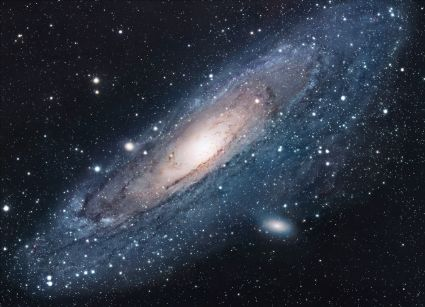
\includegraphics[scale=1.7]{figures/universe.jpg}
%   \caption{The Universe}
%   \label{Fig:universe}
% \end{figure}

\subsection{Related Work}
Robots play an important part in medical service. The International Federation of Robotics (IFR) has four major classifications of medical robots, namely: rehabilitation robots, surgical robots, assistive robots and service robots. Common medical service robots include transportation service robots in medical places and disinfection service robots.
% \begin{figure}[htbp] 
% \centering 
% 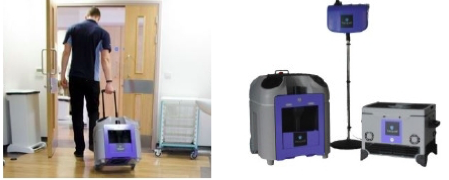
\includegraphics[width=0.4\textwidth]{figures/WechatIMG346.png} 
% \caption{Bioquell BQ-50} 
% \label{bq50} 
% \end{figure}
BQ-50 intelligent hydrogen peroxide gas generator launched by the British company Bioquell has been scientifically certified to provide solutions for air and surface pollution. It realizes one-key automatic sterilization operation\cite{rowan2020unlocking}. This product is mainly used in few wards of hospitals. The equipment is connected to the console, and the entire sterilization process can be monitored through the two buttons on the console. 
% \begin{figure}[h] 
% \centering 
% 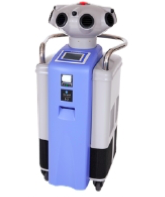
\includegraphics[width=0.2\textwidth]{figures/WechatIMG347.png} 
% \caption{Bioquell Z2} 
% \label{z2} 
% \end{figure}
Bioqull’s latest generation product Bioquell Z2 uses hydrogen peroxide gas to effectively sterilize a certain range. The unique dual-loop technology can quickly and efficiently purify the indoor environment without the need for environmental protection. 
% \begin{figure}[h] 
% \centering 
% 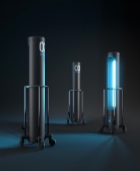
\includegraphics[width=0.2\textwidth]{figures/WechatIMG348.png} 
% \caption{Surfacide Helios} 
% \label{sh} 
% \end{figure}

    % \begin{figure}[htbp]
    % \centering
    % \begin{minipage}[t]{0.24\textwidth}
    % \centering
    % 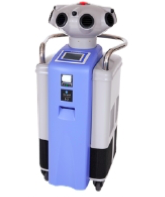
\includegraphics[width=3cm]{figures/WechatIMG347.png}
    % \caption{Bioquell Z2}
    % \label{z2}
    % \end{minipage}
    % \begin{minipage}[t]{0.24\textwidth}
    % \centering
    % 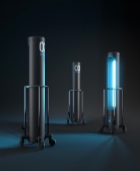
\includegraphics[width=3cm]{figures/WechatIMG348.png}
    % \caption{Surfacide Helios}
    % \label{sh}
    % \end{minipage}
    % \end{figure}

 
Surfacide UV disinfection system, developed by a UK company, has changed the previous single application mode of UV disinfection technology in the healthcare sector\cite{bedell_buchaklian_perlman_2016}. By implementing multiple light emitters in the hospital environment, it overcomes the inherent problems of incomplete disinfection caused by the use of a single UV emitter system that is easily restricted by conditions such as shadows and distance.


In general, according to the current research, ultraviolet disinfection still needs to be work in an unmanned environment but no sufficient research on the coverage of disinfection currently. Therefore, this article focus on the precise fixed point and complete coverage of alcohol spray and disinfection tasks. Meanwhile, the use of alcohol disinfection ensures that the robot disinfection and the staff perform work at the same time.

\section{System Design and Integration}\label{Sec:method}

% {\color{red}\textbf{Proposal:}}
% \begin{itemize}
%     \item In a concise way, present your solution and why you believe 
% this will improve upon the state-of-the-art. Include any 
% hardware and software proposal (either existing or new one) 
% that can be created/used for solving your problem.
% \end{itemize}

Through the background investigation, we found that good disinfection robots or medical robots should meet the characteristics of efficient work and flexible actions. We will also complete the system design according to the general needs and cognition of disinfection robots in the industry\cite{1717783}.

\subsection{Disinfection Robot Architecture Design}
\subsubsection{Mobile Base}
The base of a robot determines its flexibility, carrying capacity, and compact design. Because it needs to work in a complex and crowded environment, it is important to choose a suitable robot platform. According to the background investigation, we found that most medical robots are tall and thin, which helps them to work more like humans in sometimes crowded environments.\\
Thus, we choose Three-Mecanum-Wheel Configurations of the Mobile Robot (fig.\ref{tmw}). The base arranged in a circular array uses three wheels to better balance the load. The picture shows a common three mecanum wheel configuration. From the point of view of the intersection of the lower rollers, these configurations have omnidirectional movement performance. At the same time, the orthogonal Mecanum wheel is used for rotationally symmetrical configuration, which is usually used for indoor mobile service robots and light loading robots, which is very close to our needs.
\begin{figure}[htbp] 
\centering 
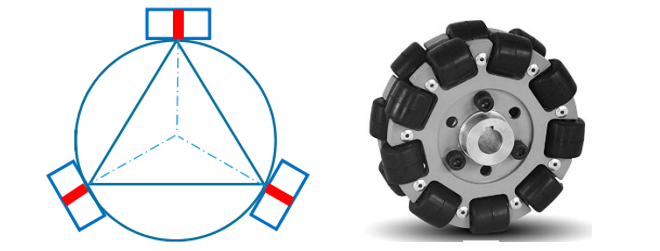
\includegraphics[width=0.45\textwidth]{figures/mwww.PNG} 
\caption{Three-Mecanum-Wheel-Base} 
\label{tmw} 
\end{figure}
\subsubsection{Robot Arm}
The reason for selecting this arm is that it can achieve full coverage and fine spraying, which effectively guarantees the coverage of disinfection, and the high DoF of the arm can ensure this. Thus, we choose to use Panda Robotic Arm\cite{gmbh_2021}, made by Franka Emika. There are several reasons for choosing it. First, it has a maximum load of 3.3kg, which satisfies the opportunity for us to perform secondary design on the end-effector of the arm. Secondly, its radius of activity is 855 mm, which satisfies the radius of most objects needed to disinfect in the hospital. At the same time, it can be perfectly compatible with ROS, and call SDKs such as movieit, which makes development convenient. Finally, after horizontal comparison, its cost performance is the highest, which also meets the requirements of large-scale production.\\
\par The overall structure is similar to RB-1 robotics (fig.\ref{rb-1}) created by Robotnik company\cite{rb-1robotnik2021}, but the Base should change to the one with Mecanum Wheels. Meanwhile, the alcohol container and hydraulic device required by spray gun will be installed on the back of the robot. There is also be a camera used for scanning modeling at the top, and the gyroscope and camera needed by SALM will be placed in front of the platform for identification. We will also install a circle of ultraviolet lights around the circular site, illuminating the ground at a designed angle, which is more conducive to the disinfection of the floor.
\begin{figure}[htbp] 
\centering 
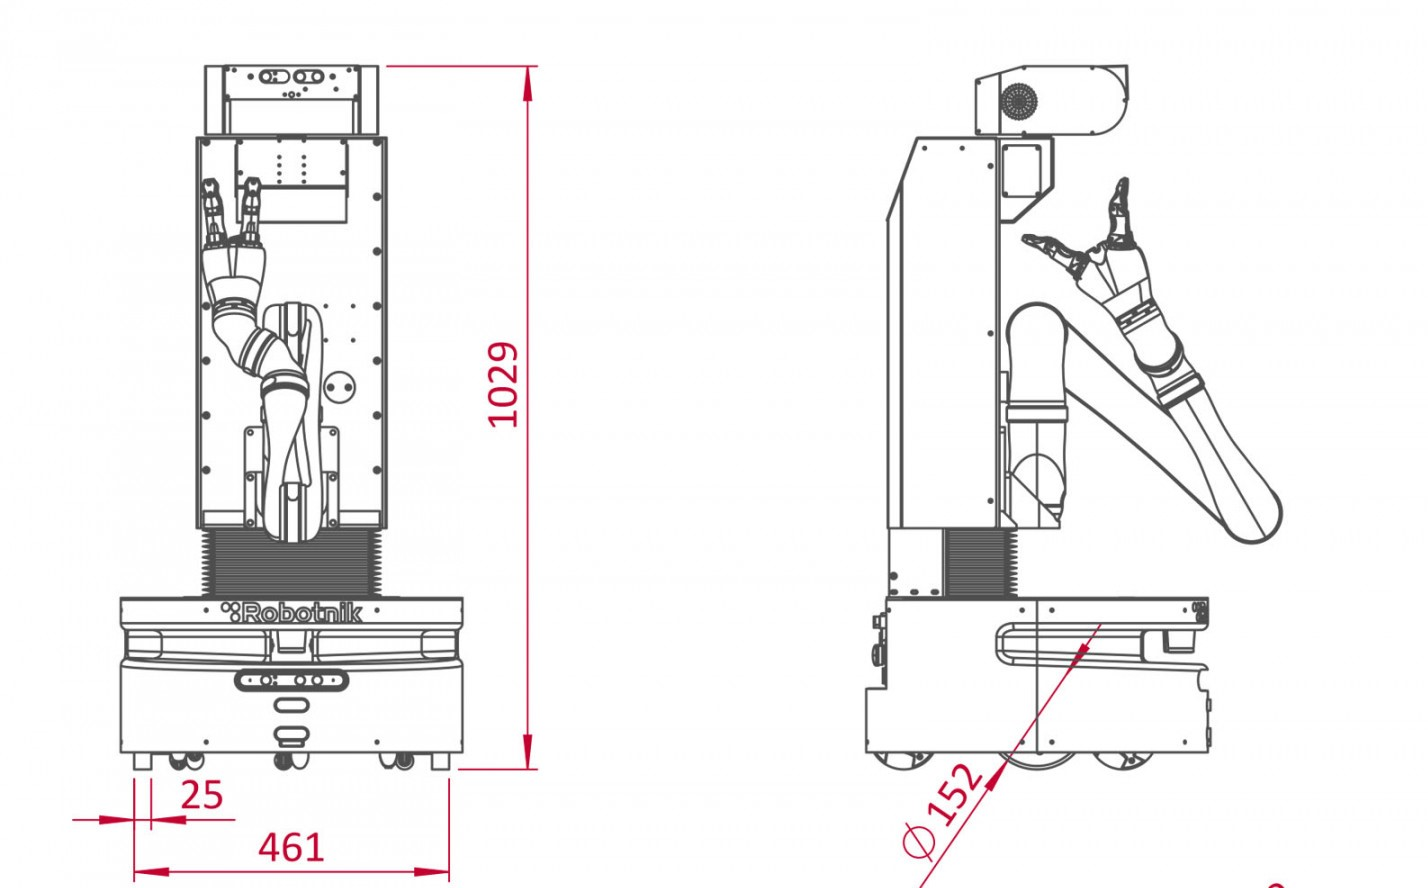
\includegraphics[width=0.45\textwidth]{figures/Robotnik-Cotas-RB-1-uai-1440x1387.jpg} 
\caption{RB-1 MOBILE MANIPULATOR} 
\label{rb-1} 
\end{figure}
\subsection{Movement Planning}
For a disinfection robot that automatically works in a hospital, mapping and localization are the basic requirements. Nowadays SLAM(Simultaneous Localization and Mapping) is an advanced and hottest technology to deal with this issue. Since SLAM was first proposed 30 years ago \cite{pritsker1984introduction}, it has gone through rapid development. In the future, the development of multi-sensors SLAM \cite{zhang2013application} and Semantic SLAM \cite{bowman2017probabilistic} can greatly improve the accuracy of mapping and localization which are good enough for the robot's work.
\par Also, the robot needs motion planning. It is divided into two parts, global planning and local planning. Global planning refers to a route that the robot moves on. Local planning refers to adjust itself when there are accidents during the movement. So far, to realize more complicated functions of service robot which is required to move in a more specific route and back to recharge when the battery is low, a topic named space coverage is researcher, one of the most famous algorithm and theory is called Morse Decompositions \cite{acar2002morse}. Based on this theory, the disinfection robot can divide the space then disinfect respectfully and recharge itself. 
              

\subsection{Multi-function End-effector Design}

In order to achieve full coverage spraying, we designed a switchable end-effector. In the background investigation, we found that the spraying shape is different according to the nozzle and pressure. According to the figure.\ref{spray pattern} \cite{ikeuchi_2021},
\begin{figure}[htbp] 
\centering 
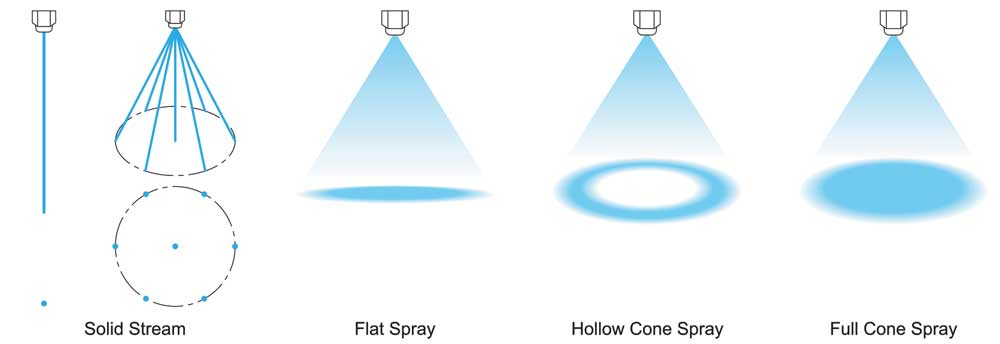
\includegraphics[width=0.5\textwidth]{figures/Spray-pattern.jpg} 
\caption{Spray Pattern} 
\label{spray pattern} 
\end{figure} 
we can see the most common spray patterns, according to different application scenarios, there will be different alcohol spraying solutions. For instance, when cleaning gaps or corners, we should use flat spray, and when spraying large areas, we should switch to a solid cone method. In order to integrate all the solutions, so as to achieve full coverage spraying, we have been inspired by the CNC machine tool and the lens converter of the microscope, and all the nozzles are assembled on a disc to form a cone, as shown in the figure.\ref{Nozzle Conversion Disc}, when the robot judges the different solutions are needed, just switch the nozzles to complete the corresponding tasks.


\begin{figure}[htbp] 
\centering 
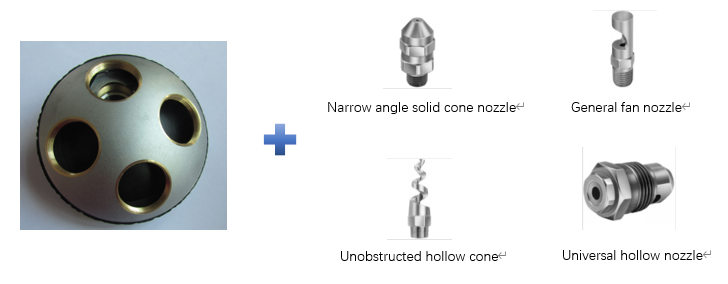
\includegraphics[width=0.5\textwidth]{figures/translator.PNG} 
\caption{Nozzle Conversion Disc} 
\label{Nozzle Conversion Disc} 
\end{figure}

\subsection{3D Scan Modeling and Control Method Design}
In the medical environment, disinfection of transparent glassware or plastic cups has always been very challenging. As a full-coverage disinfection robot, we have borrowed from the ClearGrasp algorithm(fig.\ref{3dshape})\cite{sajjan2020clear}, which is a deep learning method used to learn from a single RGB-D Estimate the accurate 3D geometry of transparent objects in the image for robot manipulation. Given an RGB-D image of a single transparent object, ClearGrasp uses a deep convolutional network to infer surface normals, masks and occlusion boundaries for transparent surfaces. These outputs are then used to optimize the initial depth estimate for all transparent surfaces in the scene. 
\par After obtaining the object model needed to spray and disinfect, we should plan the spraying path through graphic algorithms, which, analyzing the approximate shape of the object, and judge the edges and faces. Then manipulate the arms and the ground to reach these areas for work. Among algorithms for full-coverage scanning of known modeling. We recommend using DJI's PTZ fixed-point tracking algorithm\cite{dji}, which can identify the following objects in the air and follow the shooting 360 degrees. Applied it to our scene, it can spray around the known object from top to bottom so that cover all the exposed area of the object.
\begin{figure}[htbp] 
\centering 
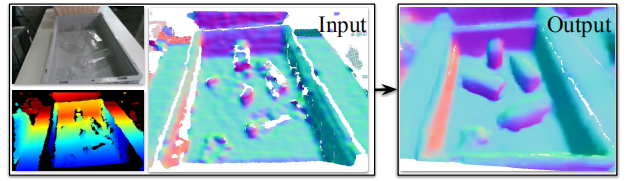
\includegraphics[width=0.45\textwidth]{figures/2020clear.png} 
\caption{3D Shape Estimation of Transparent Objects} 
\label{3dshape} 
\end{figure}
\section{Hypothesis and Evaluation}\label{Sec:evaluation}

\par In order to detect the accuracy of precise point and complete full coverage of alcohol spray and disinfection, the coverage rate is introduced as the evaluation index of robot disinfection. Fluorescent reagents are used instead of alcohol in the experiment to visualize the coverage. After the experiment is over, detect the objects to be disinfected and the fluorescent reagents in the experimental scene to evaluate the accuracy of the disinfection. The experiment will be carried out as follows.
\par The experiment will be divided into two parts, the first part detects precise point disinfection, and the second part detects complete coverage of disinfection. First, create an experimental scene, a confined space about 40 square meters in size, including two rooms A and B. Place an experiment table in the two rooms, and place an object to be disinfected on the two experiment tables, for example, an ornament. At the same time, obstacles are placed in each room to detect the obstacle avoidance function of the robot. After starting the robot, the robot will enter rooms A and B in turn to carry out disinfection work. The scope of disinfection includes the entire house and objects to be disinfected. After the robot returns to its original position after the disinfection work is completed, the coverage rate of the fluorescent reagent in the room and the coverage rate of the fluorescent reagent on the surface of objects are detected to evaluate the accuracy of detecting precise points and complete coverage of alcohol spray and disinfection, respectively.





\section{Conclusions and Future Work}\label{Sec:concl}
To control the severe spreading\cite{spreading} of COVID-19 and reduce the heavy labor cost in this pandemic, disinfection plays an important role. A new type of disinfection robot is designed. It provides a solution for precise fixed-point and full coverage alcohol spraying disinfection.

The designed robot is a combination of a mobile base and robot arm with an alcohol sprayer as an end-effector. Three-Mecanum-Wheel Configurations is the mobile base to make the robot suitable for working in a medical environment. As for the robot arm, the structure is identical to that of RB-1. Regarding its motion, SLAM is applied for localization and mapping, and algorithms like Morse Decompositions and ClearGrasp are inserted for solving various situations of a robot such as avoiding unexpected obstacles and recognizing transparent objects.

In the future, methods for disinfection can be explored further,such as ultralviolet used in UVD robots.\cite{FLEMING2018241} End-effector which is an alcohol sprayer currently, should able to be replaced by other devices such as ultralviolet light, realizing disinfection with higher efficiency.
With the development of modern society, the human-robot interaction is a focus and can be explored further under well-designed research the medical robotics.\cite{medicalkansei} According to the concept of Kansei engineering\cite{kansei}, some elements of our robot perhaps can be replaced by other structures or material under the circumstance of maintaining the original function. 

\bibliographystyle{IEEEtran}
\bibliography{references}



% {\color{red} Red Parts need to be determined, \textbf{DDL is 3.10}, Each one should take one to write(Both Introduction and Background belong \ref{Sec:intro}),\textbf{ IF WE CAN'T HANDLE, WE SHOULD EXTEND IT!!!!!! SO GUYS MAKE DECISION AS SOON AS POSSIBLE!}}
\end{document}

